% Q12 -- Pseudo-static RAM cell. Dynamic storage node written through a write TG (phi1);
% a feedback inverter loop closed by a second TG (phi2) refreshes/recirculates the value;
% an output buffer inverter drives Q. NOTE: the notes have no dedicated pseudo-static RAM
% cell, so this applies the pseudo-static principle (dynamic storage + auto-refresh).
\documentclass[border=10pt]{standalone}
\usepackage{tikz}
\usetikzlibrary{arrows.meta,shapes.geometric}
\begin{document}
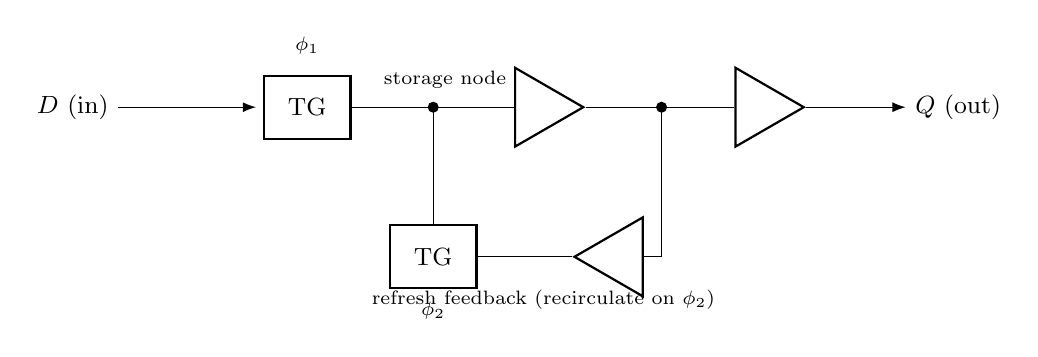
\begin{tikzpicture}[>=Latex, font=\small]
% input D
\draw[->] (-2.4,0) node[left]{$D$ (in)} -- (-0.65,0);
% write transmission gate (phi1)
\node[draw, thick, minimum width=1.1cm, minimum height=0.8cm] (tg1) at (0,0) {TG};
\node[above, font=\scriptsize] at (0,0.55) {$\phi_1$};
% storage node
\draw (tg1.east) -- (1.6,0) coordinate (sn);
\fill (sn) circle (2pt);
\node[above, font=\scriptsize] at (1.75,0.12) {storage node};
% forward inverter
\node[draw, thick, isosceles triangle, isosceles triangle apex angle=60,
      minimum width=1cm] (inv1) at (2.9,0) {};
\draw (sn) -- (inv1.west);
% node X
\draw (inv1.east) -- (4.5,0) coordinate (x);
\fill (x) circle (2pt);
% output buffer inverter
\node[draw, thick, isosceles triangle, isosceles triangle apex angle=60,
      minimum width=1cm] (inv2) at (5.7,0) {};
\draw (x) -- (inv2.west);
\draw[->] (inv2.east) -- (7.6,0) node[right]{$Q$ (out)};
% feedback inverter (points left) + slave TG (phi2) -> refresh loop back to storage node
\node[draw, thick, isosceles triangle, isosceles triangle apex angle=60,
      minimum width=1cm, shape border rotate=180] (invf) at (4.0,-1.9) {};
\node[draw, thick, minimum width=1.1cm, minimum height=0.8cm] (tg2) at (1.6,-1.9) {TG};
\node[below, font=\scriptsize] at (1.6,-2.35) {$\phi_2$};
\draw (x) -- (4.5,-1.9) -- (invf.east);
\draw (invf.west) -- (tg2.east);
\draw (tg2.north) -- (sn);
\node[font=\scriptsize] at (3.0,-2.45) {refresh feedback (recirculate on $\phi_2$)};
\end{tikzpicture}
\end{document}
